\documentclass{article}

\usepackage{fancyhdr, lastpage}
\usepackage[inline]{enumitem}
\usepackage{listings}
\usepackage[scaled=0.95]{inconsolata}  % Use a monospaced font, like Inconsolata
\usepackage{wasysym}
\usepackage{booktabs}
\usepackage{booktabs, multicol, multirow, array, threeparttable}
\usepackage{siunitx}
\usepackage{xfrac}
\usepackage{extramarks}
\usepackage{amsmath, amsthm, amsfonts, mathtools, empheq}
\usepackage{caption}
\usepackage[table]{xcolor}
\usepackage{tikz}
\usepackage[most]{tcolorbox}
\usepackage{pagecolor} %% for dark background
\usepackage{hyperref}
\usepackage{refcount}


\topmargin=-0.45in
\evensidemargin=0in
\oddsidemargin=0in
\textwidth=6.5in
\textheight=9.0in
\headsep=0.25in

\linespread{1.1}

% Define a command to print last page number without hyperlink
\newcommand*{\lastpagewithoutlink}{%
    \getpagerefnumber{LastPage}%
}

\pagestyle{fancy}
\lhead{\hmwkAuthorName}
\chead{\hmwkTitle}
\rhead{\hmwkClass}
\lfoot{\lastxmark}
\cfoot{Page \thepage \ of \lastpagewithoutlink}


\renewcommand\headrulewidth{0.4pt}
\renewcommand\footrulewidth{0.4pt}

\setlength\parindent{0pt}

%
% Create Problem Sections
%

\newcommand{\enterProblemHeader}[1]{
    \nobreak\extramarks{}{Problem \arabic{#1} continued on next page\ldots}\nobreak{}
    \nobreak\extramarks{Problem \arabic{#1} (continued)}{Problem \arabic{#1} continued on next page\ldots}\nobreak{}
}

\newcommand{\exitProblemHeader}[1]{
    \nobreak\extramarks{Problem \arabic{#1} (continued)}{Problem \arabic{#1} continued on next page\ldots}\nobreak{}
    \stepcounter{#1}
    \nobreak\extramarks{Problem \arabic{#1}}{}\nobreak{}
}

\setcounter{secnumdepth}{0}
\newcounter{partCounter}
\newcounter{homeworkProblemCounter}
\setcounter{homeworkProblemCounter}{1}
\nobreak\extramarks{Problem \arabic{homeworkProblemCounter}}{}\nobreak{}

%
% Homework Problem Environment
%
% This environment takes an optional argument. When given, it will adjust the
% problem counter. This is useful for when the problems given for your
% assignment aren't sequential. See the last 3 problems of this template for an
% example.
%
\newenvironment{homeworkProblem}[1][-1]{
    \ifnum#1>0
        \setcounter{homeworkProblemCounter}{#1}
    \fi
    \section{Problem \arabic{homeworkProblemCounter}}
    \setcounter{partCounter}{1}
    \enterProblemHeader{homeworkProblemCounter}
}{
    \exitProblemHeader{homeworkProblemCounter}
}

%
% Homework Details
%   - Title
%   - Due date
%   - Class
%   - Section/Time
%   - Instructor
%   - Author
%

\newcommand{\hmwkTitle}{Homework\ \#4}
\newcommand{\hmwkDueDate}{April 20, 2024}
\newcommand{\hmwkClass}{EGR 5110}
\newcommand{\hmwkClassTime}{}
\newcommand{\hmwkClassInstructor}{Professor Nissenson}
\newcommand{\hmwkAuthorName}{\textbf{Francisco Sanudo}}

%
% Title Page
%

\title{
    \vspace{2in}
    \textmd{\textbf{\hmwkClass:\ \hmwkTitle}}\\
    \normalsize\vspace{0.1in}\small{Due\ on\ \hmwkDueDate\ at 11:59pm}\\
    \vspace{0.1in}\large{\textit{\hmwkClassInstructor\ \hmwkClassTime}}
    \vspace{3in}
}

\author{\hmwkAuthorName}
\date{}

\renewcommand{\part}[1]{\textbf{\large Part \Alph{partCounter}}\stepcounter{partCounter}\\}

%
% More settings
%

% Table Settings
% \setlength{\tabcolsep}{5pt} % Gap before text starts
\renewcommand{\arraystretch}{2.5} % Cell Height Scaling
\setlength{\arrayrulewidth}{0.5mm} % Table Border Thickness
\arrayrulecolor{blue} % Table Border Color
\newcolumntype{s}{>{\columncolor{black!10}} c}

% Link Settings
\hypersetup{
    colorlinks=false,       % false: boxed links; true: colored links
    linkcolor=red,          % color of internal links (change box color with linkbordercolor)
    citecolor=green,        % color of links to bibliography
    urlcolor=cyan,           % color of external links
    pdftitle={EGR 5110 HW3}
}

% Color defintions
\definecolor{magenta}{RGB}{255,0,255}
\definecolor{cyan}{RGB}{0,255,255}
\definecolor{white}{RGB}{255,255,255}
\definecolor{red}{RGB}{255,0,0}
\definecolor{green}{RGB}{0,255,0}
\definecolor{orange}{RGB}{255,165,0}
\definecolor{yellow}{RGB}{255,255,0}
\definecolor{blue}{RGB}{10,10,255}

% Text color shortcuts
\newcommand{\cw}{\color{white}}
\newcommand{\cm}{\color{magenta}}
\newcommand{\cc}{\color{cyan}}
\newcommand{\cred}{\color{red}}
\newcommand{\cb}{\color{blue}}
\newcommand{\cg}{\color{green}}
\newcommand{\cy}{\color{yellow}}
\newcommand{\co}{\color{orange}}

%
% Various Helper Commands
%


% For derivatives
\newcommand{\deriv}[2]{\frac{d#1}{d#2}}

% For partial derivatives
\newcommand{\pderiv}[2]{\displaystyle \frac{\partial #1}{\partial #2}}

% Redefine \dfrac if you want all fractions to be in display style automatically
\newcommand{\ddfrac}[2]{\frac{\displaystyle #1}{\displaystyle #2}}

% Alias for the Solution section header
\newcommand{\solution}{\textbf{\large Solution}}

%% Box settings
% \setlength{\fboxsep}{9pt} % Adjust the padding thickness here
\setlength{\fboxrule}{1pt} % Adjust the border thickness here

% The \dimexpr\linewidth-2\fboxsep-2\fboxrule\relax calculation ensures that the width of the minipage is reduced by twice the padding and twice the border width, as there is padding and border on both the left and right sides.
\newcommand{\boxsettings}{\dimexpr\linewidth-2\fboxsep-2\fboxrule\relax}

% Paragraph box shortcut for tables
\newcommand{\PB}[2]{\parbox{#1}{\centering #2}}




\begin{document}

\maketitle

\pagebreak

\section{Background}
A long rectangular fin is attached to a heat source. The fin is much longer (into the page) than its other
dimensions, so heat flow is approximately two-dimensional. Its left side is subjected to a constant base
temperature of 100 ${}^{\circ}$C and the other three sides experience convection. The fin's initial temperature is\\ 
40 ${}^{\circ}$C and the free stream air temperature is 25 ${}^{\circ}$C. \\

Below is a cross sectional view of the fin:

\begin{figure}[h]
    \centering
    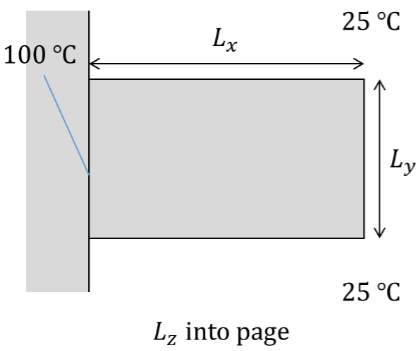
\includegraphics[width=0.3\textwidth]{fig/fin.png}
    \caption{Long Rectangular Fin Attached to Heat Source}
    \label{fig:fin}
\end{figure}

The time-dependent temperature distribution is governed by the 2D heat diffusion equation

\begin{equation}
    \pderiv{T}{t} = \alpha \left( \pderiv{^2 T}{x^2} + \pderiv{^2 T}{y^2}\right)
    \label{eq:2DHeat}
\end{equation}
where $T$ is temperature and $\alpha$ is the thermal diffusivity coefficient.\\

\textbf{Goal}: Solve Equation~\eqref{eq:2DHeat} from an initial time $t_0$ to a final time $t_f$ for the temperature distribution across the 2D rectangular fin in Figure~\ref{fig:fin} (as a function of time) using a finite-difference method.

\pagebreak

\section{Deriving Node Equations}

\pagebreak

\section{Scenarios}

\begin{table}[h]
    \centering
    \caption{Five Scenarios Using an Explicit Finite-Difference Method}
    \small
    \begin{threeparttable}
        \begin{tabular}{|s|c|c|c|c|c|c|c|c|} \hline
            {\cellcolor{yellow!50} \bf Scenario} & {\PB{1cm}{$k_{\textrm{cond}}$\\$\left(\frac{\textrm{W}}{\textrm{m} \, {}^{\circ}\textrm{C}}\right)$}} & {\PB{1.3cm}{$\alpha$\\$\left(\frac{\textrm{m}^2}{\textrm{s}}\right)$}} & {\PB{1.1cm}{$h$\\$\left(\frac{\textrm{W}}{\textrm{m}^2 \, {}^{\circ}\textrm{C}}\right)$}} & {\PB{1cm}{$t_{ss}$\\(min)}} & {\PB{1.3cm}{$T_{\textrm{avg}}$ tip\\1D eqn* (${}^{\circ}$C)}} &  {\PB{1.3cm}{$T_{\textrm{avg}}$ tip\\sim* (${}^{\circ}$C)}} & {\PB{1.3cm}{$\dot{Q}$\\1D eqn* (W)}} & {\PB{1.3cm}{$\dot{Q}$\\sim* (W)}}
            \\ \hline
            Pure Al, fan high   & 240 & \SI{97e-6}{} & 100 & 0.93 & 93.94 & 94.16 & 133.31 & 126.32      \\ \hline
            Pure Al, fan low    & 240 & \SI{97e-6}{} & 10  & 0.99 & 99.35 & 99.37 & 14.02 & 13.27   \\ \hline
            AISI 302  &  15 & \SI{4e-6}{} & 100 & 11.23 & 52.54 & 53.57 & 78.49 & 74.32 \\ \hline
            Low $k$, high $\alpha$  & 3 & \SI{100e-6}{} & 100  & 0.055 & 28.77 & 29.40 & 37.61 & 34.43  \\ \hline
            High $k$, low $\alpha$  & 100 & \SI{3e-6}{} & 100  & 27.51 & 86.72 & 87.18 & 124.08 & 117.68  \\  \hline
        \end{tabular}
        \label{tab:Scenarios}
        \begin{tablenotes}
            \item [*] The average tip temperature and heat rate are the values at the end of the simulation, which are well past the time when the contour lines stop moving.
        \end{tablenotes}
    \end{threeparttable}
\end{table}

\pagebreak

\begin{figure}[h]
    \centering
    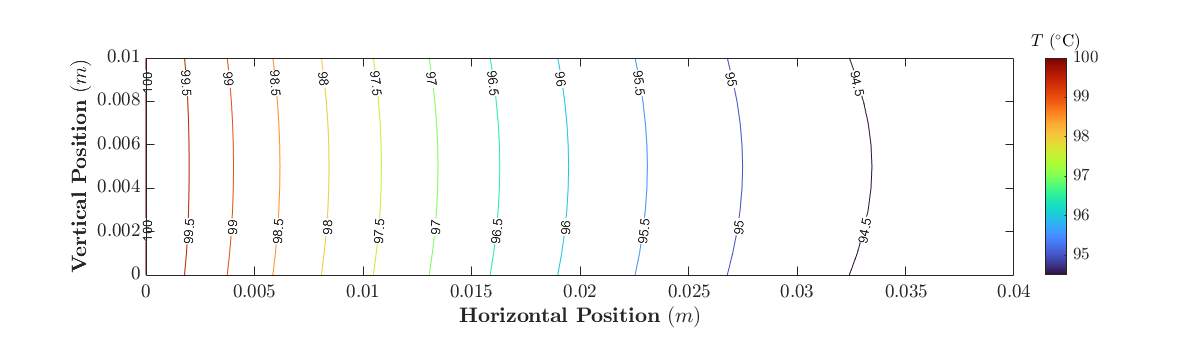
\includegraphics[width=1\textwidth]{fig/contour1.png}
    \caption{Steady-State Temperature Distrubution for Scenario 1}
    \label{fig: Plot1}
\end{figure}

\pagebreak

\begin{figure}[h]
    \centering
    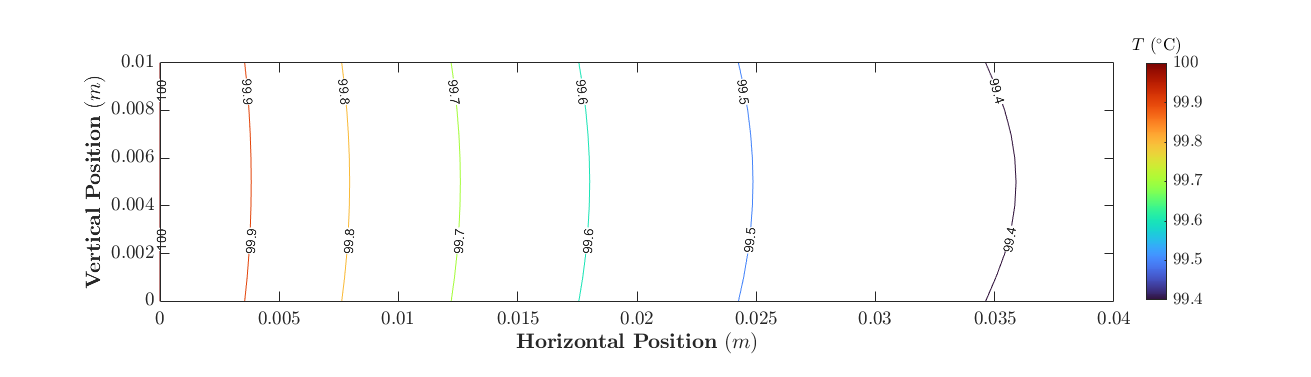
\includegraphics[width=1\textwidth]{fig/contour2.png}
    \caption{Steady-State Temperature Distrubution for Scenario 2}
    \label{fig: Plot2}
\end{figure}

\pagebreak

\begin{figure}[h]
    \centering
    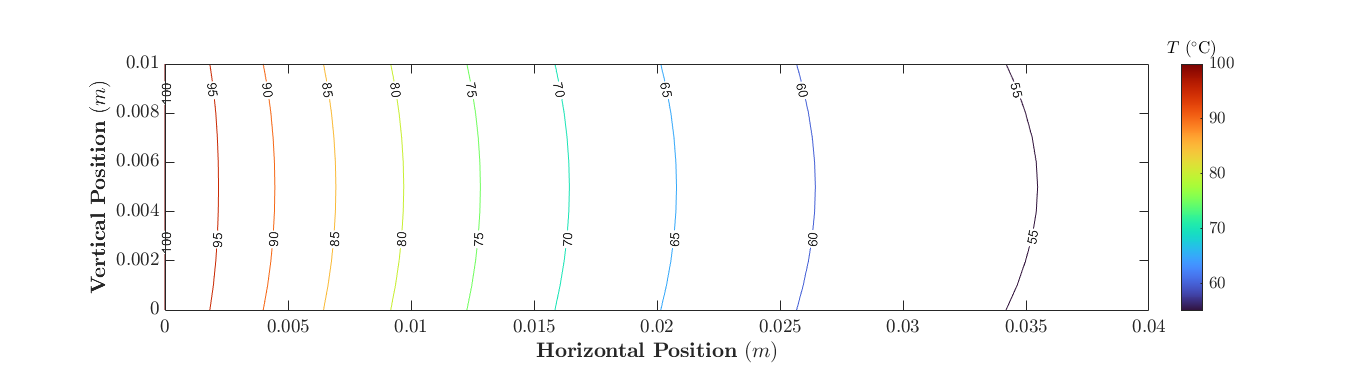
\includegraphics[width=1\textwidth]{fig/contour3.png}
    \caption{Steady-State Temperature Distrubution for Scenario 3}
    \label{fig: Plot3}
\end{figure}

\pagebreak

\begin{figure}[h]
    \centering
    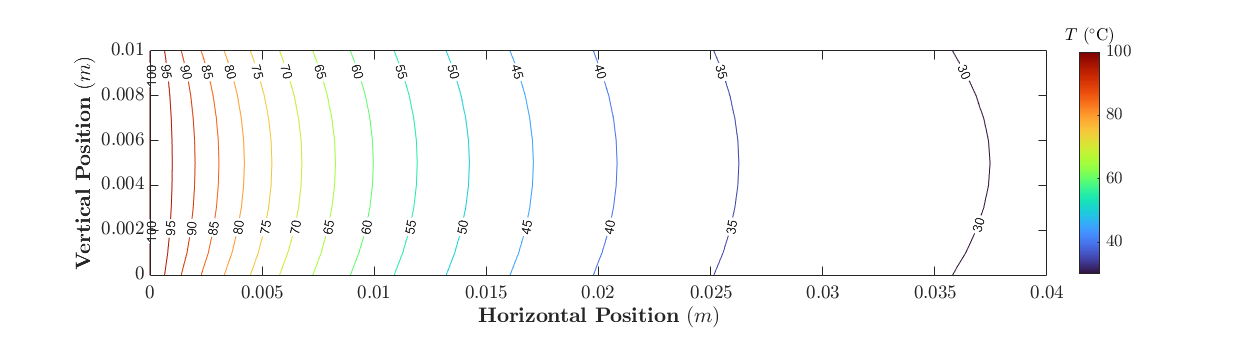
\includegraphics[width=1\textwidth]{fig/contour4.png}
    \caption{Steady-State Temperature Distrubution for Scenario 4}
    \label{fig: Plot4}
\end{figure}

\pagebreak

\begin{figure}[h]
    \centering
    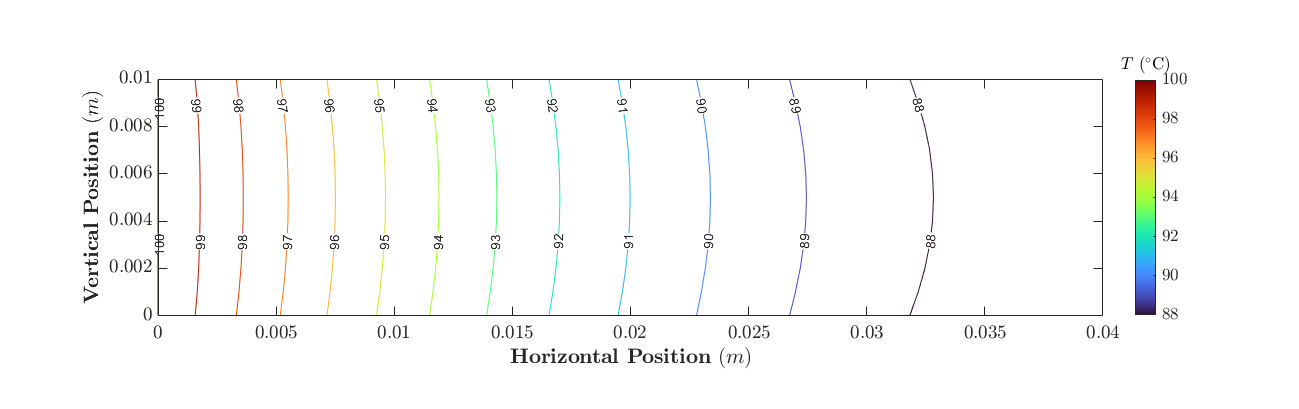
\includegraphics[width=1\textwidth]{fig/contour5.png}
    \caption{Steady-State Temperature Distrubution for Scenario 5}
    \label{fig: Plot5}
\end{figure}


\end{document}
